\NewChapter{信存者}

\quote{我通过观察,发现了那些柔弱的病者,亲眼目睹它们不能继续享用蜜汁,不能进食,渐渐地,一点点憔悴下去,衰弱下去。}{《昆虫记》}

在核战争后的世界,一切都化为了荒芜。世界的秩序早已破碎不堪,一切活物的目标都只剩下生存。而你作为“动物们“信赖的朋友,苟活于一个逼仄的房间中,与这个世界沟通的唯一渠道就是收获信件,并且安排“动物朋友”出门探索。动物们会自由地活动,并且产生饥饿、心理疾病等状态。作为“动物们”所信赖的指挥官,尽可能地让所有的动物在残酷的战后世界中存活下来吧!

\section{创作背景}

游戏创作于2022年10月,是2022网易游戏高校Mini-Game挑战赛参赛作品。《信存者》是一款单人策略生存游戏,灵感来源为知名的核战生存游戏《60秒》。游戏内玩家将扮演避难所指挥官的角色,带着化身为动物的伙伴们生存。避难所与外界沟通的途径只有信件、包裹以及冒着风险派动物伙伴外出获取资源。性格迥异的动物伙伴、世事难料的事件、游荡冷酷的恶鬼、丰富奇特的道具,聚集伙伴的勇气和信念,生存下去吧!

\begin{figure}[H]
    \centering
    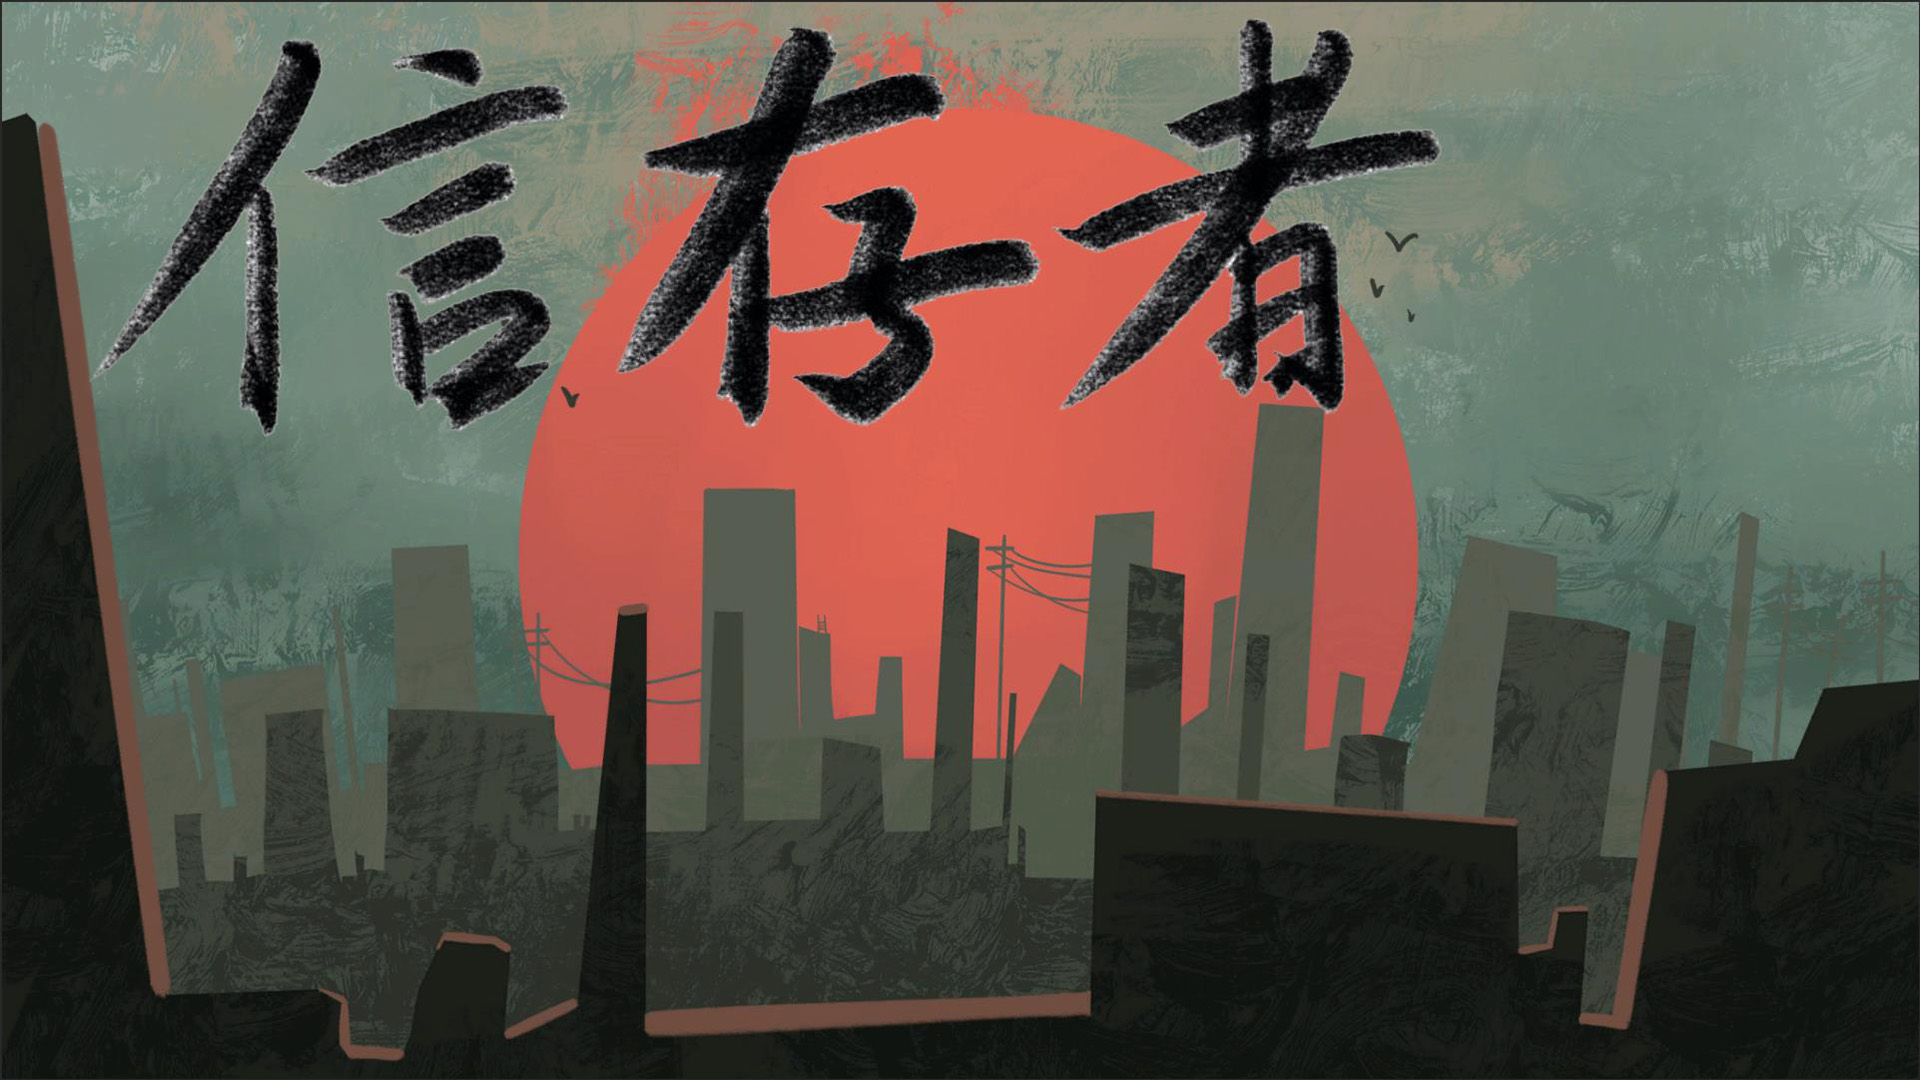
\includegraphics[width=0.8\textwidth]{Images/信存者/poster.jpg}
    \caption{信存者\ 游戏封面}
\end{figure}

\section{设计思路}
基于比赛的主题“信”,采用了具象的“信件”与意向的“相信”和“信念”作为游戏的玩法与主题。我们主要从两个核心体验入手:

\begin{enumerate}
\item \textbf{难以割舍的选择:} 在游戏中,你有着一些性格各异的“动物朋友”,TA们信赖你,所以选择你来安排一切事物。游戏的主要玩法之一是:每天,你都能获得信封与包裹,在它们当中,你会获得外界的一些动向,根据碎片的信息,你需要选择是否相信,又是否要让你的伙伴为此去探险。每个不同的选择都会触发不一样的故事与结局。

\item \textbf{运筹帷幄地经营:} 在有限的储存空间中,决定哪些物资应该留下,哪些物资必须舍弃。将有限的食物与水分配给“动物朋友”,尽量可能地保护大家存活下来。
\end{enumerate}

\begin{figure}[H]
    \centering
    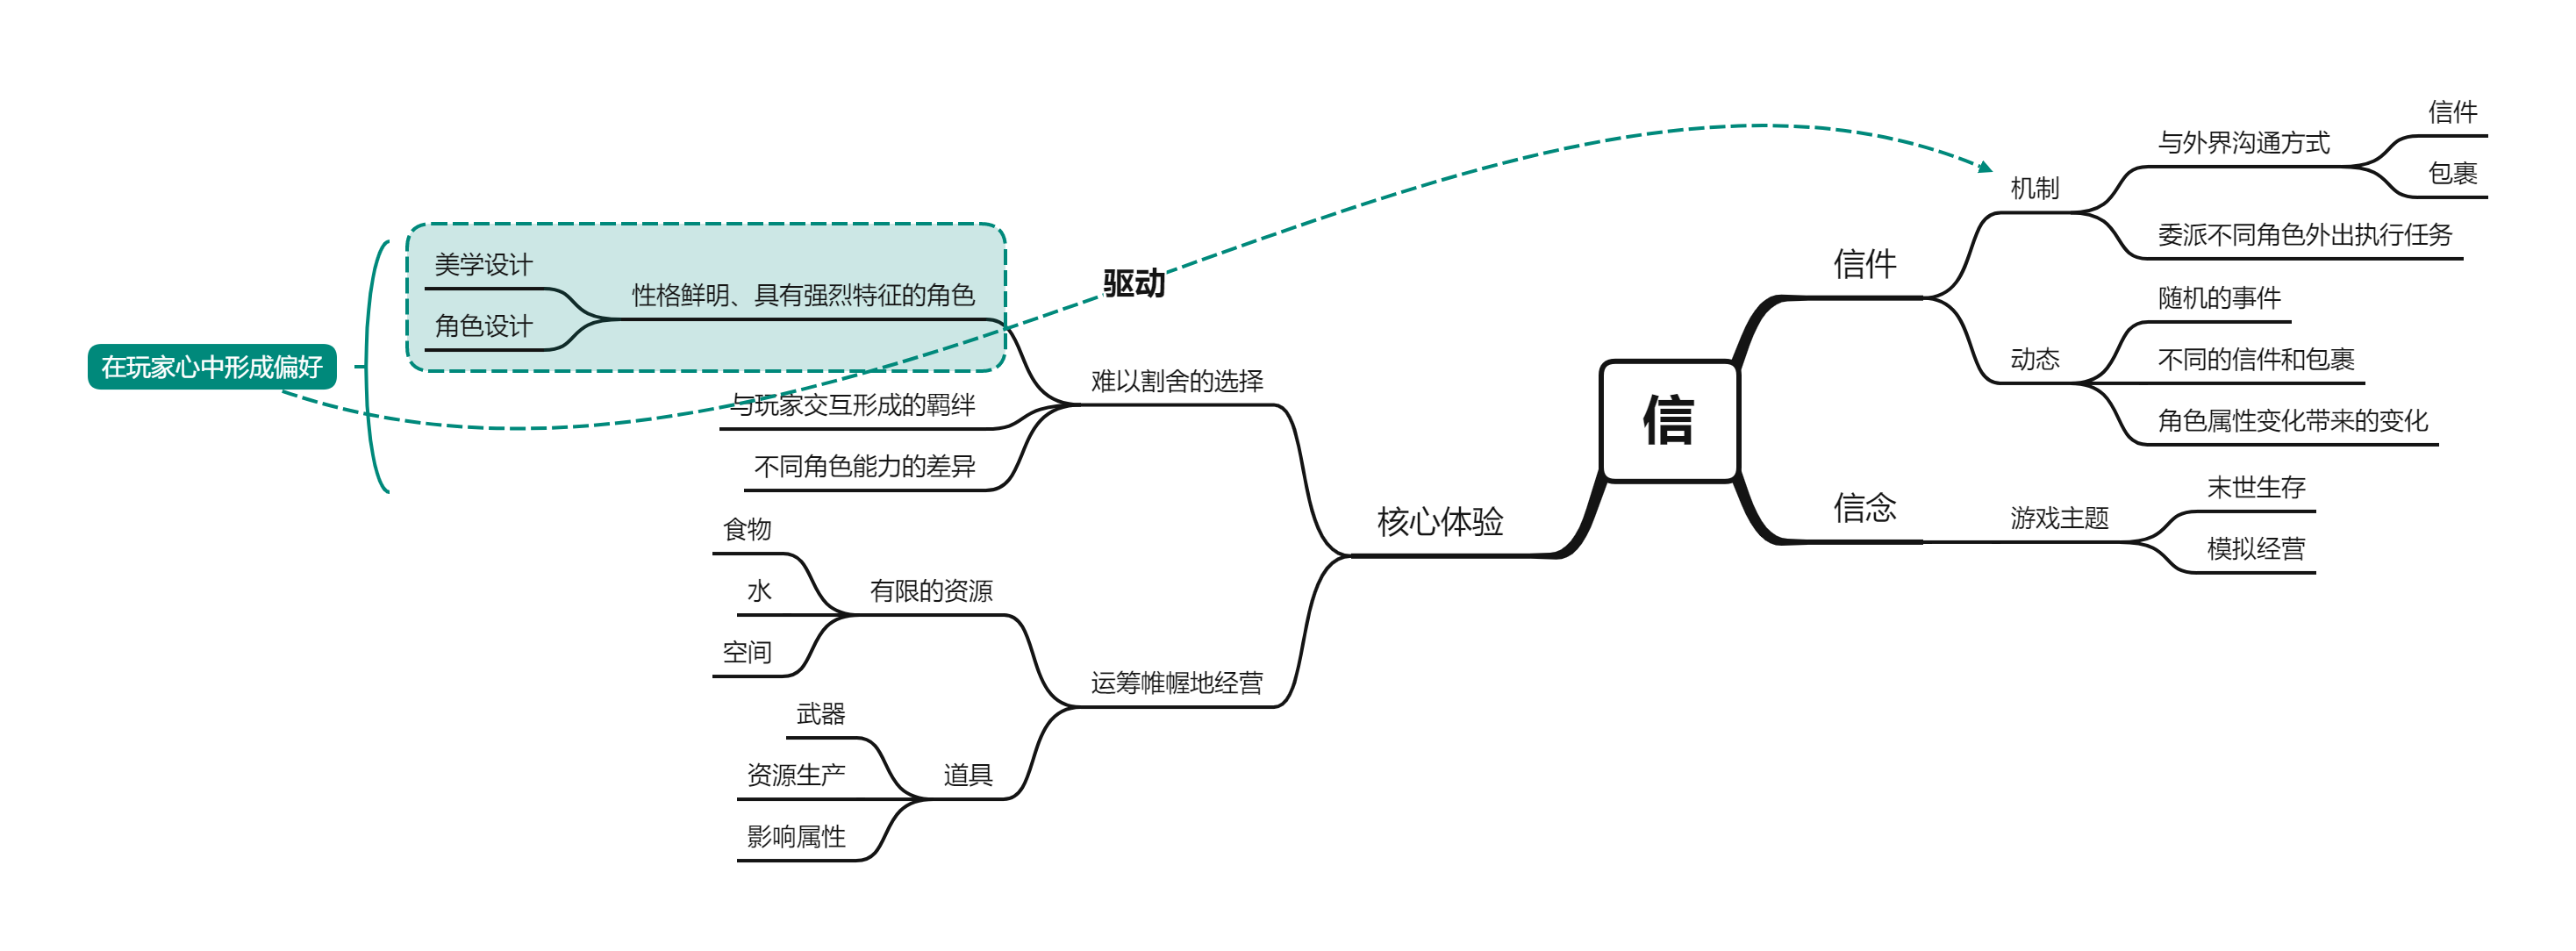
\includegraphics[width=0.8\textwidth]{Images/信存者/design.png}
    \caption{信存者\ 早期游戏拆解}
\end{figure}

我们想要营造末世中为了生存不得不做出违背良心的选择,或者为了保留心爱的角色必须牺牲其他角色的痛苦和无奈。所以人物设计以及相关的美学设计是游戏的重点。

\begin{figure}[H]
\centering  %图片全局居中
\subfigure[封面采取昏暗的置景升起代表生机的红日]{
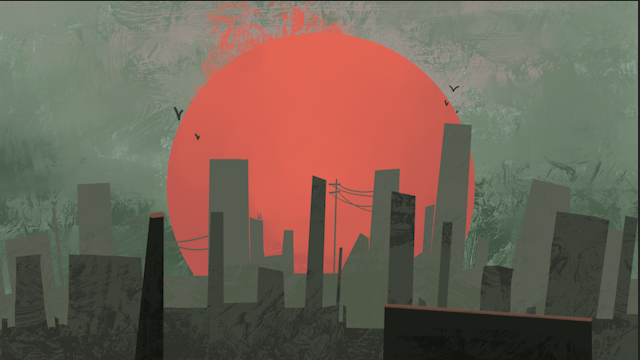
\includegraphics[width=0.45\textwidth]{Images/信存者/sun.png}}
\subfigure[长期不见天日的房间使用比较灰暗但整体和谐的黄绿色调]{
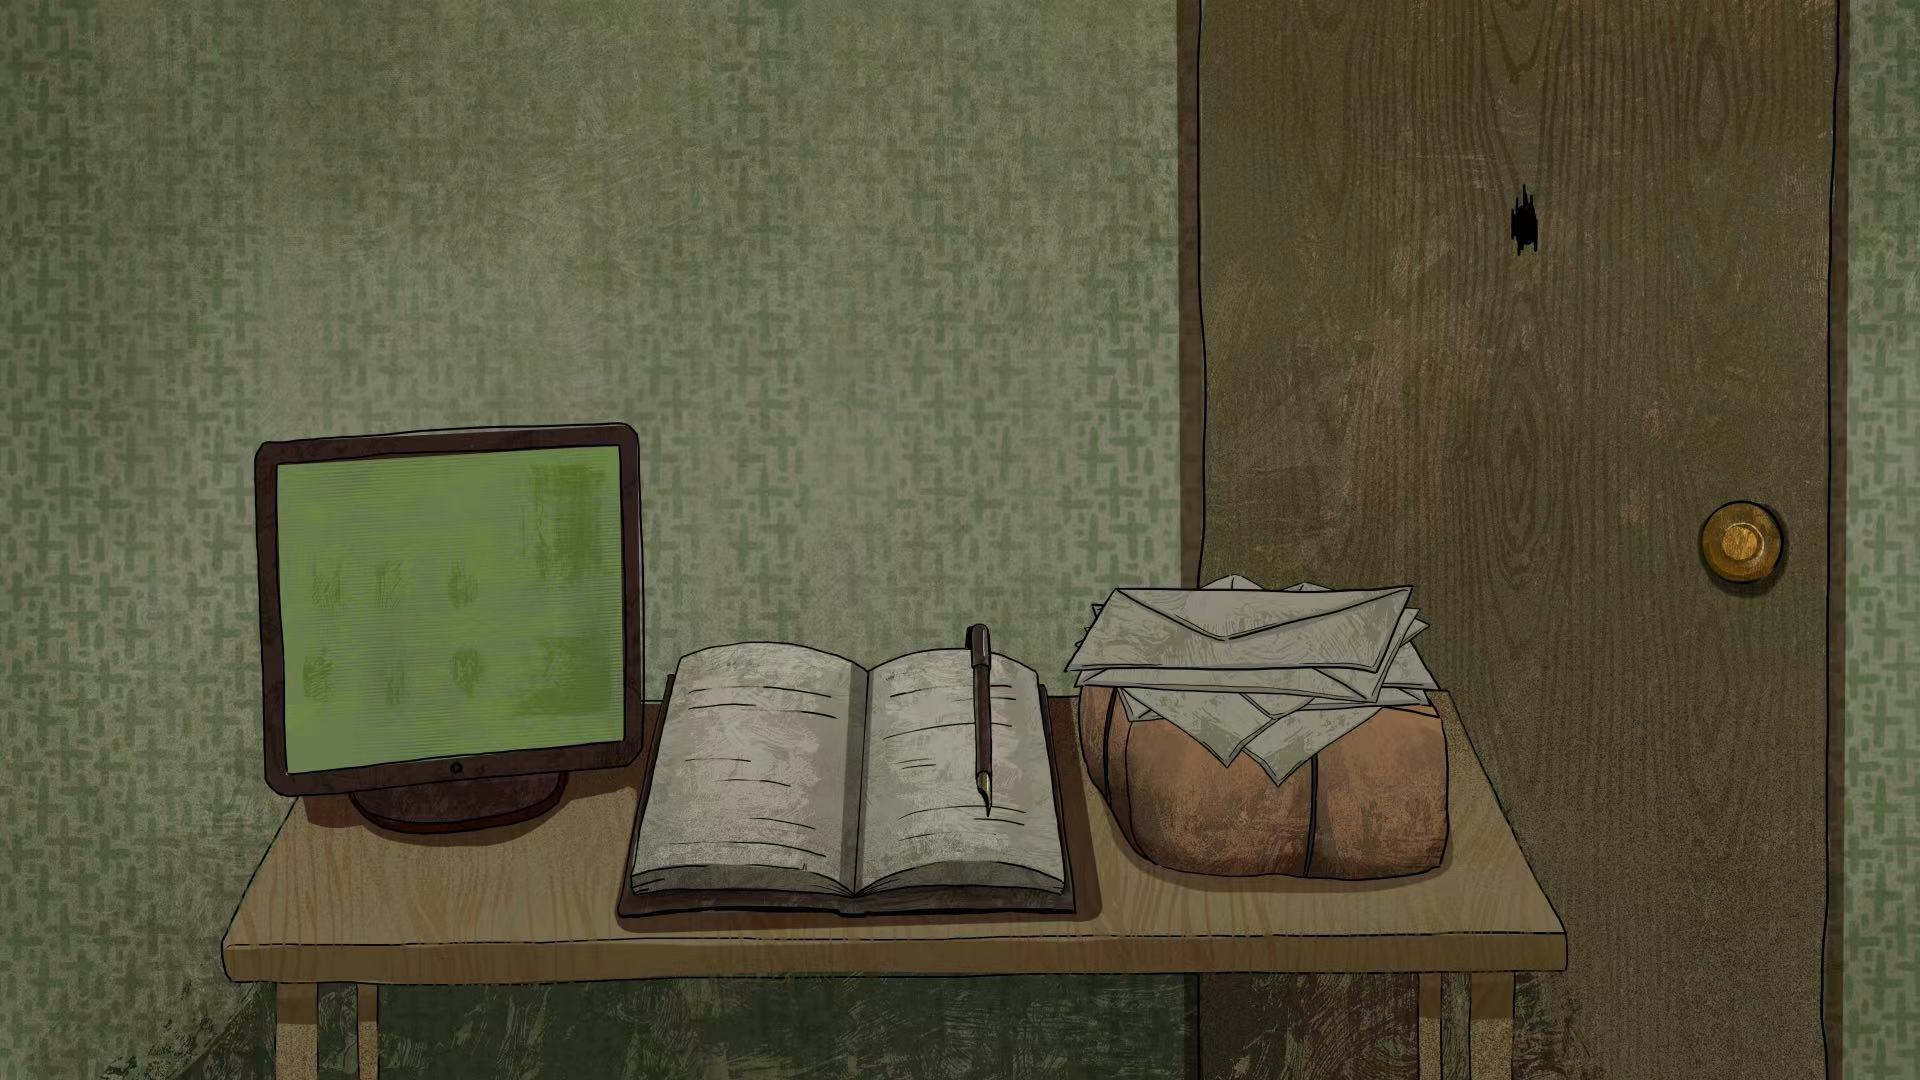
\includegraphics[width=0.45\textwidth]{Images/信存者/room.jpeg}}
\subfigure[背包和整体保持统一的色调]{

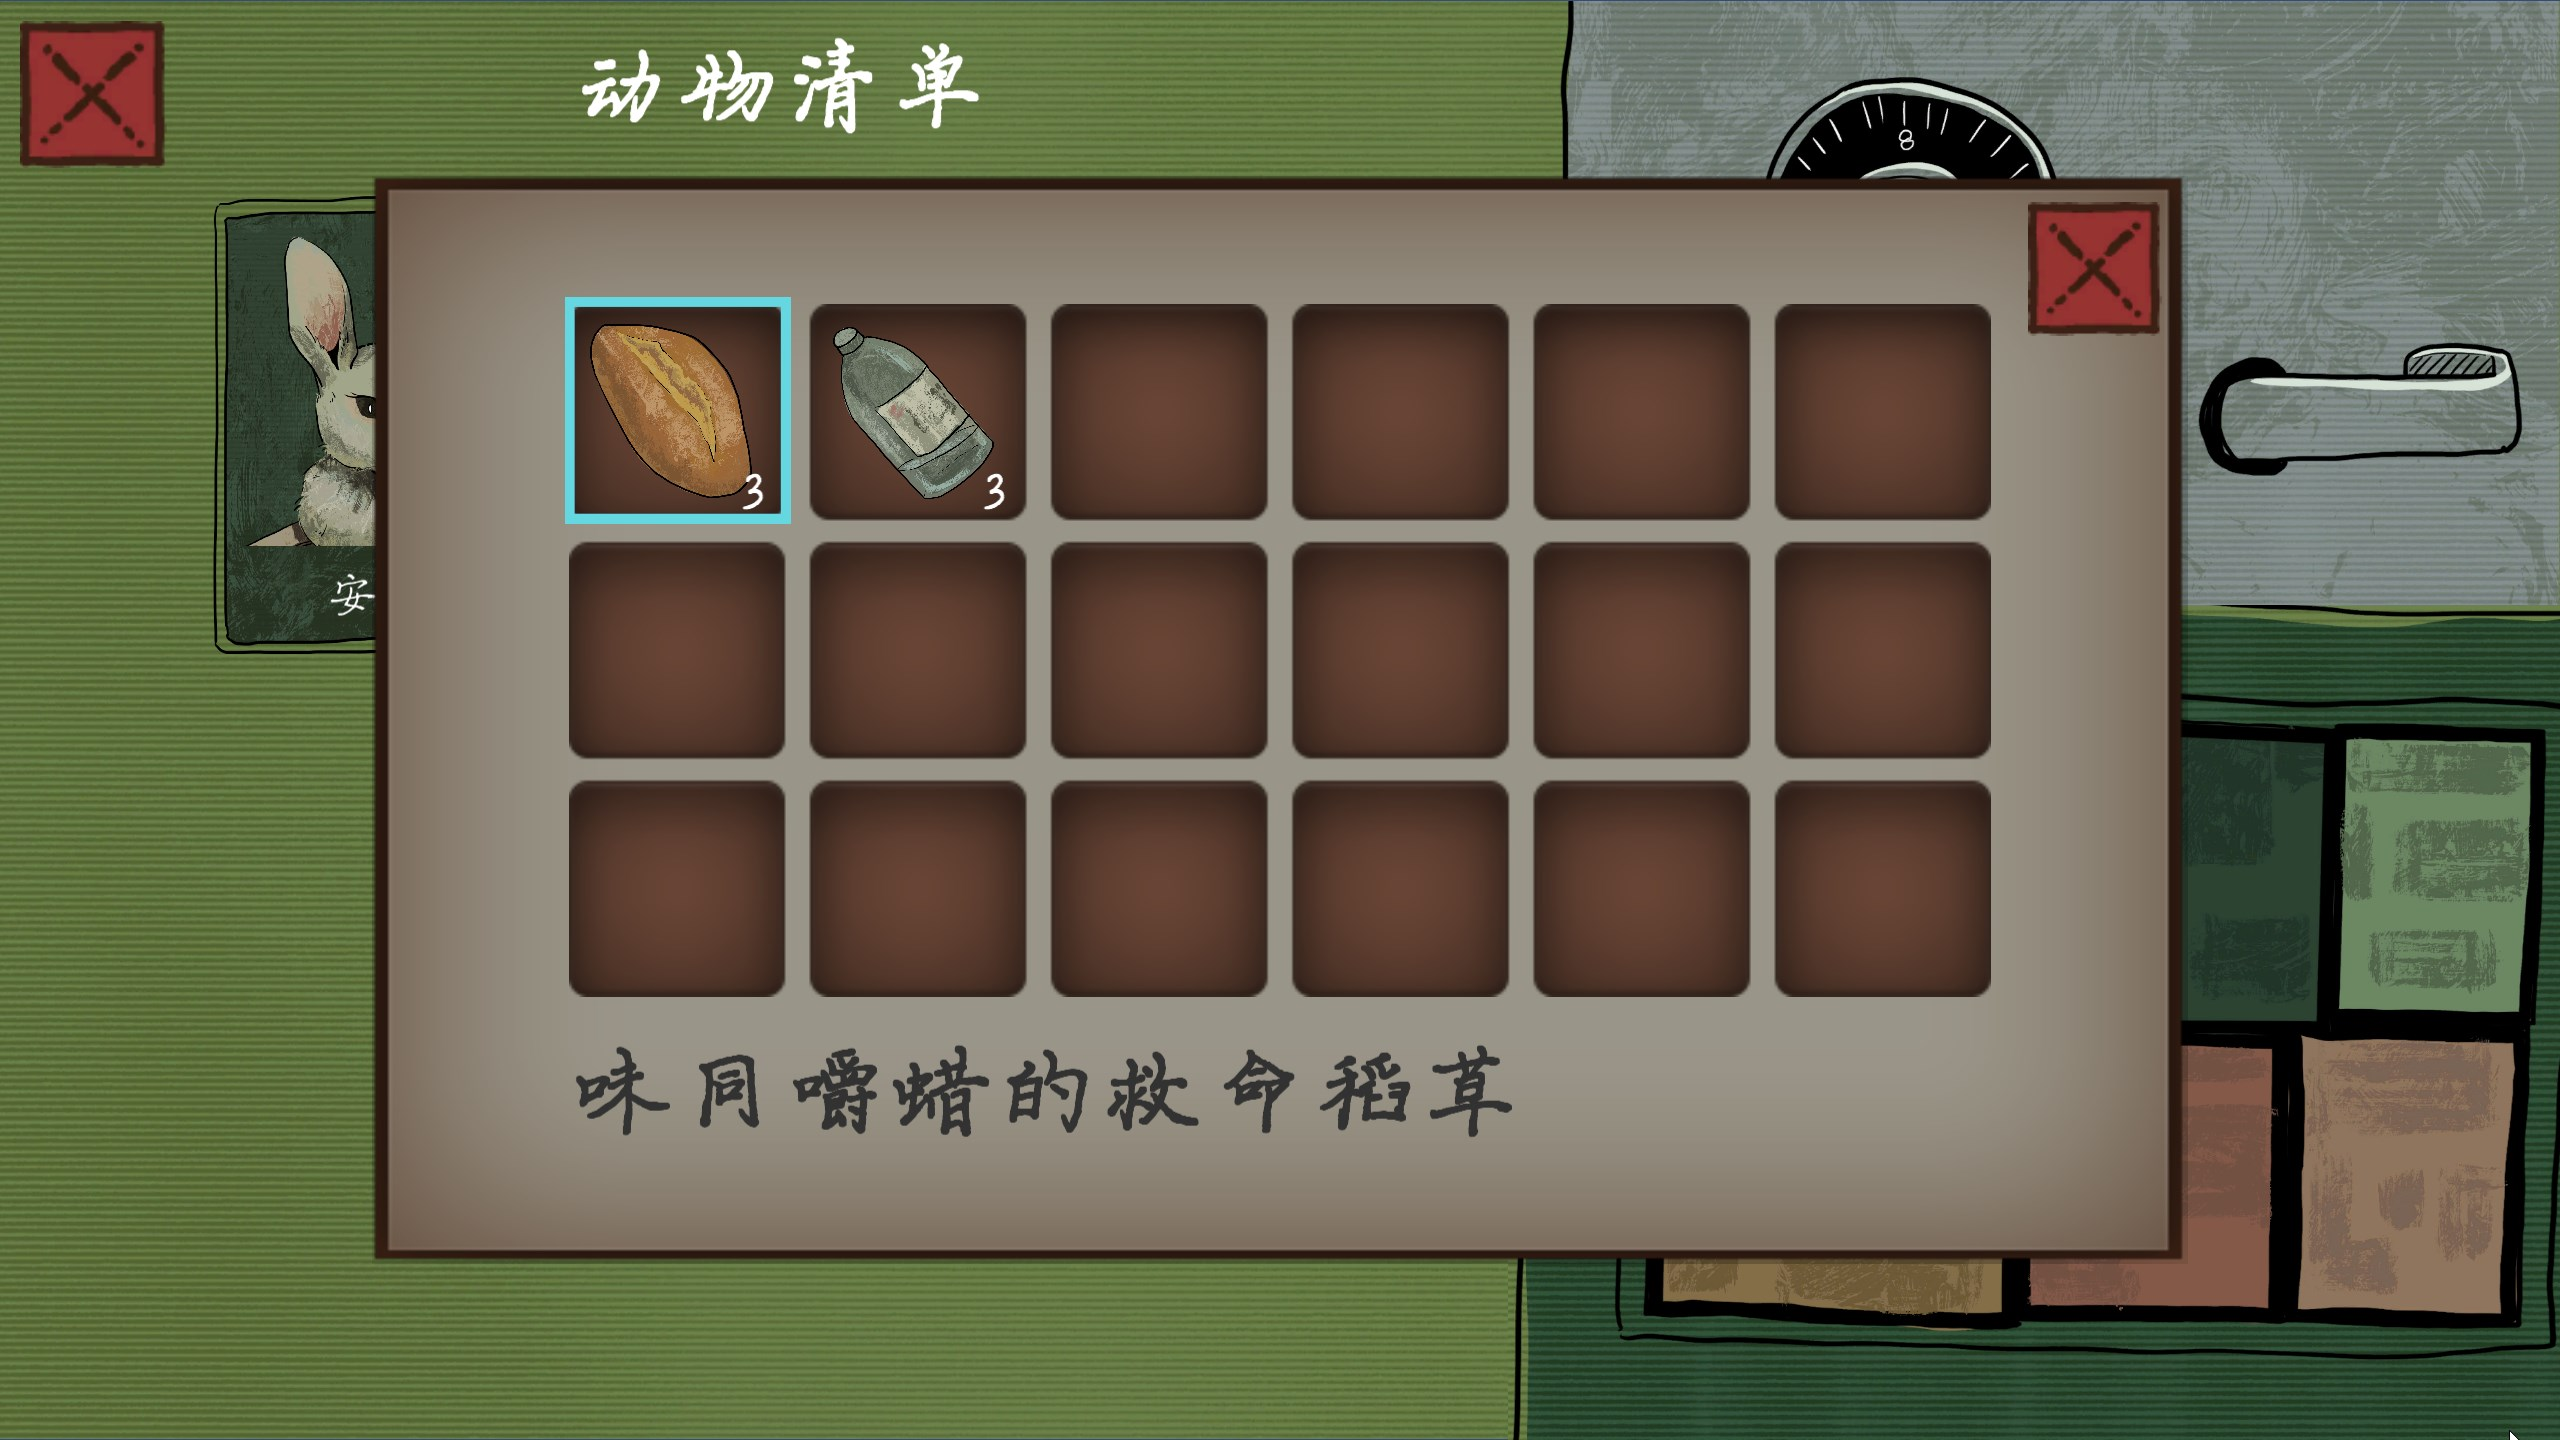
\includegraphics[width=0.45\textwidth]{Images/信存者/package.jpg}}
\subfigure[残缺的日记本记录每天的事件]{
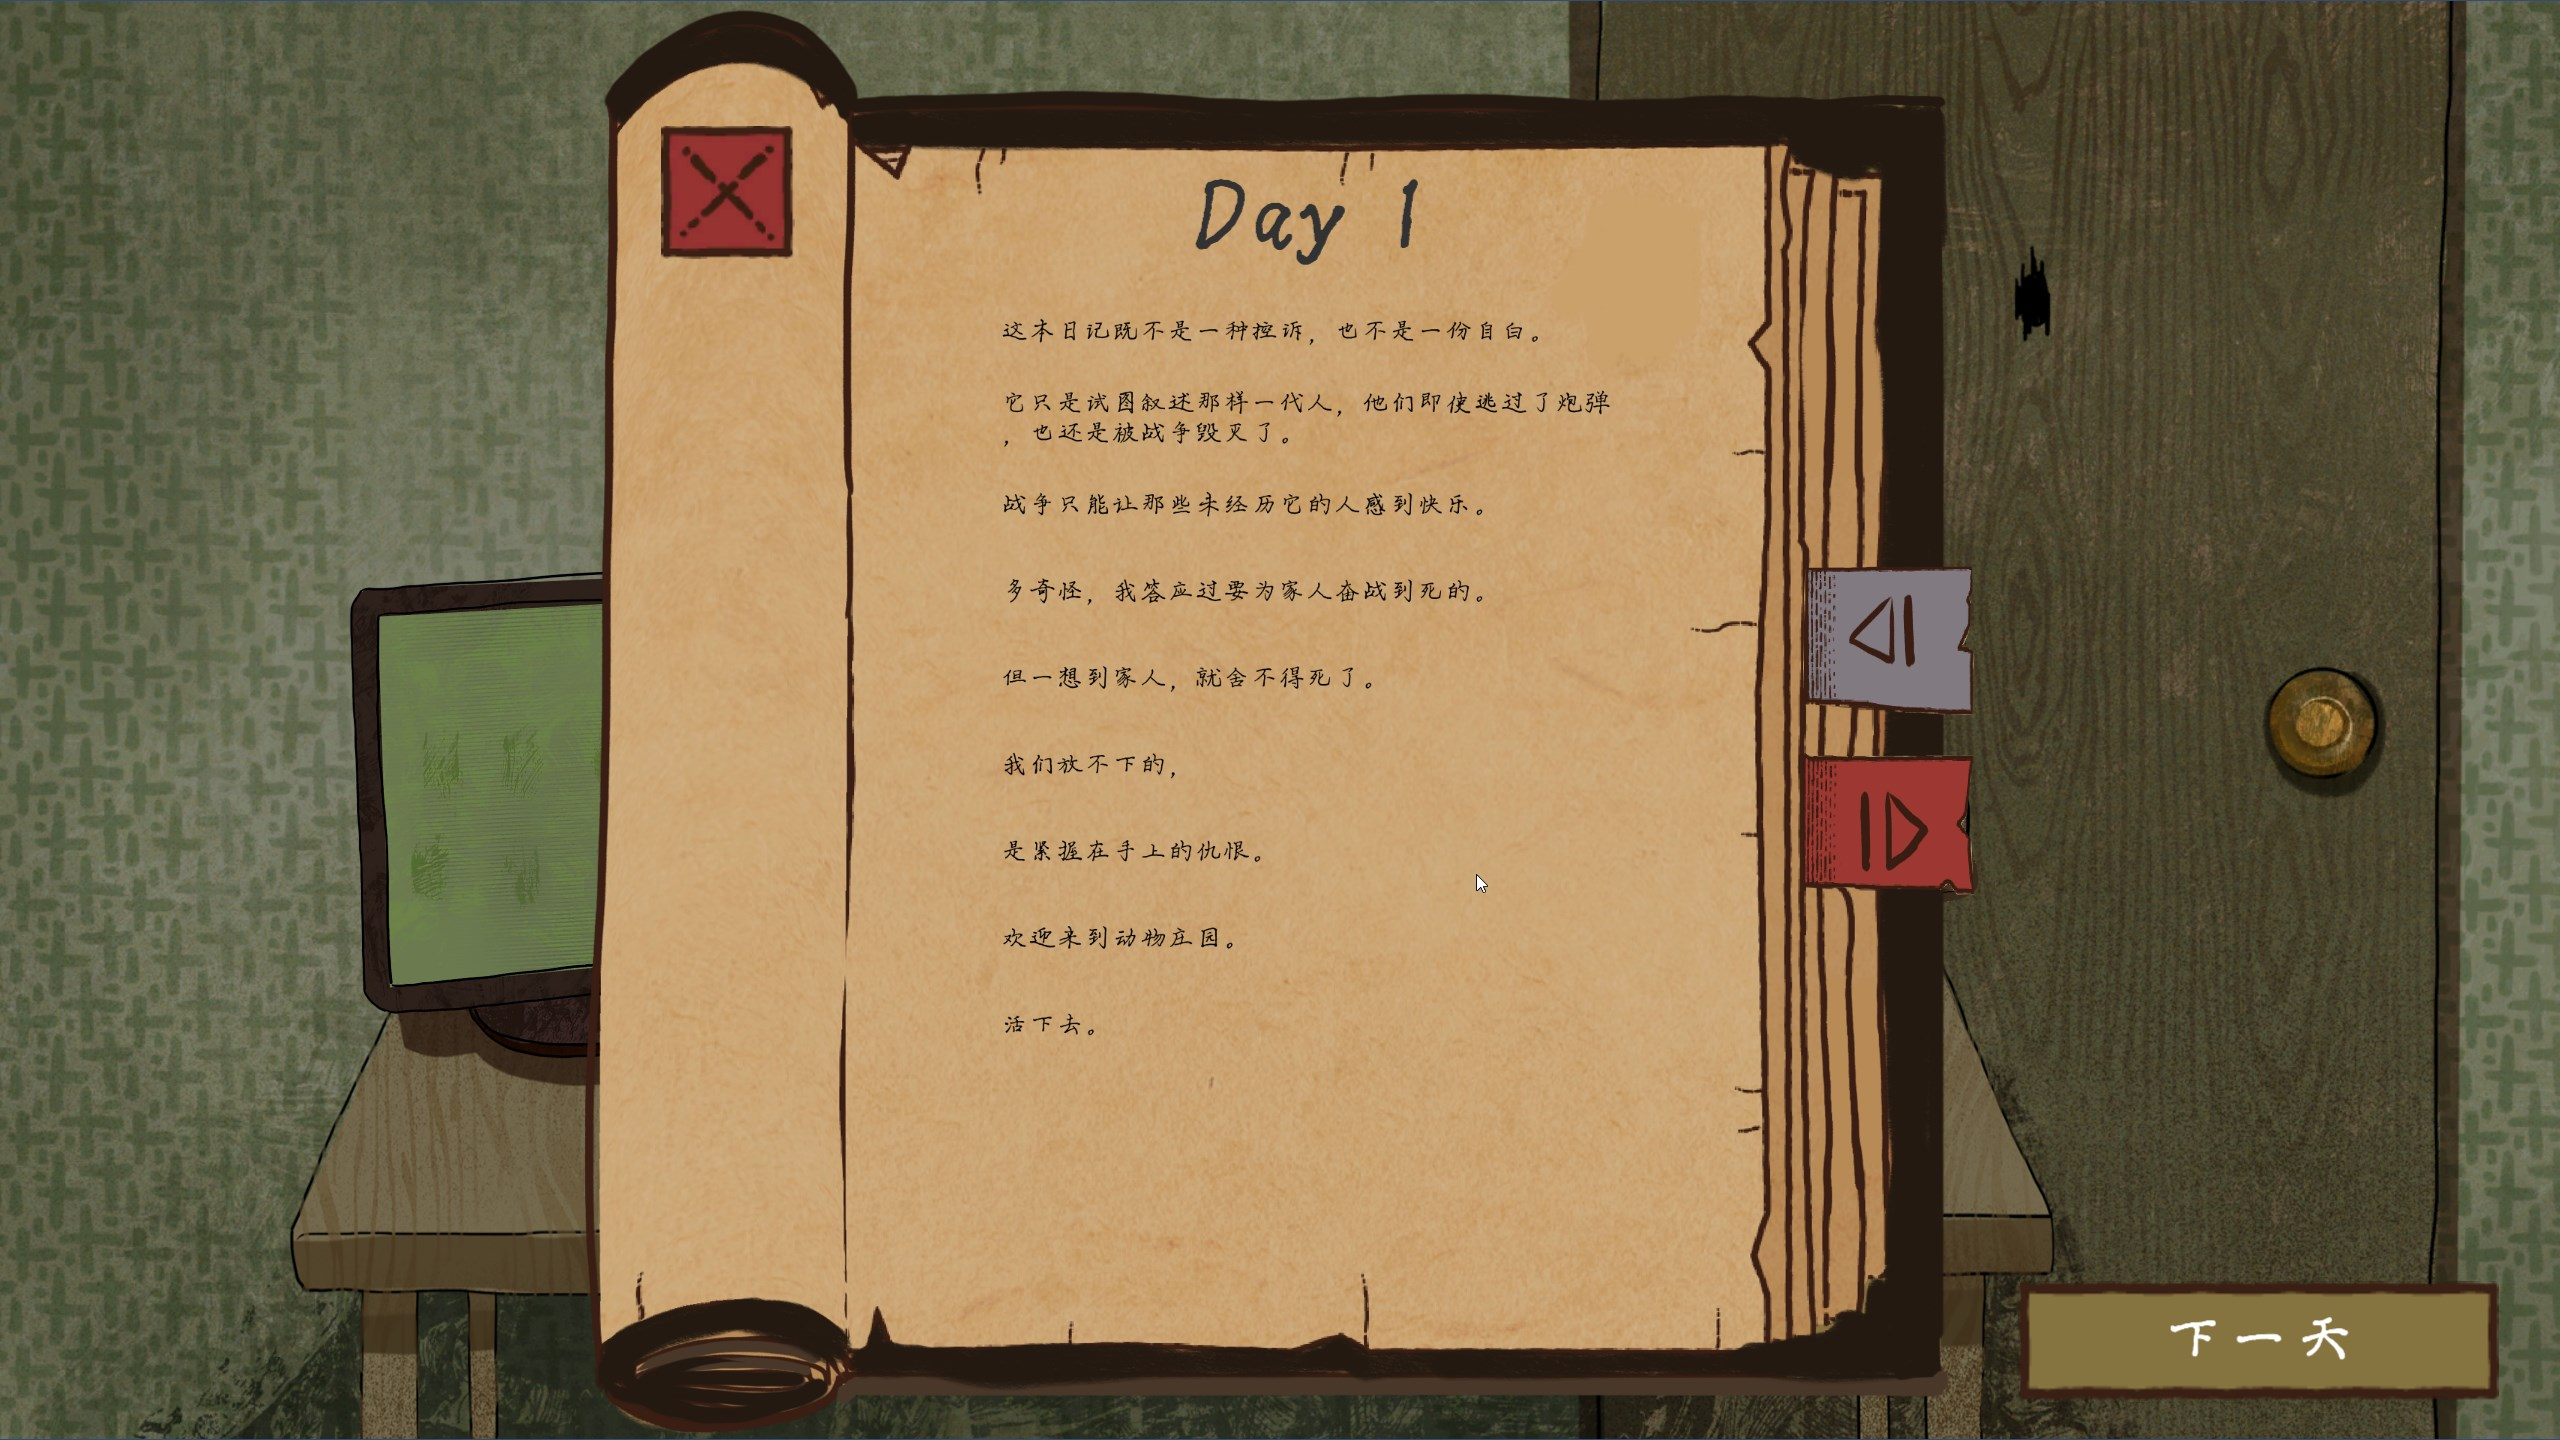
\includegraphics[width=0.45\textwidth]{Images/信存者/diary.jpg}}
\caption{沉重的“反战”、“人性”主题,色调采用灰色调的暗调}
\end{figure}

角色设计上,为了让玩家更快认识到不同的角色,从美学、性格设定上进行了一定的脸谱化设计。Demo版本一共设计了三个角色,象征冷静的兔子——安宁、象征力量的公鸡——司羽和象征活力的牧羊犬——贝。

\begin{figure}[H]
\centering  %图片全局居中
\subfigure[冷静的灰绿色]{
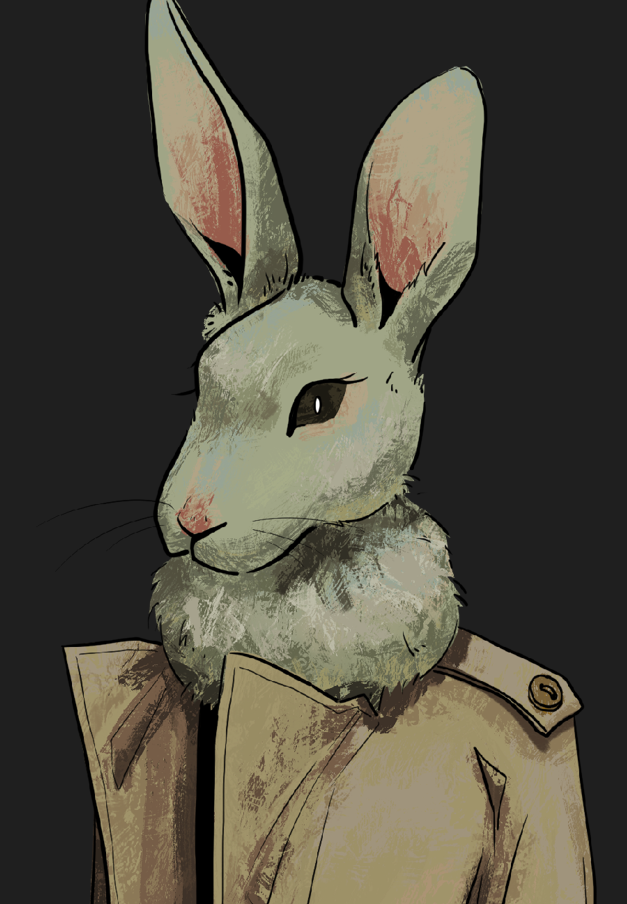
\includegraphics[width=0.3\textwidth]{Images/信存者/anning.png}}
\subfigure[桀骜的红黄色]{
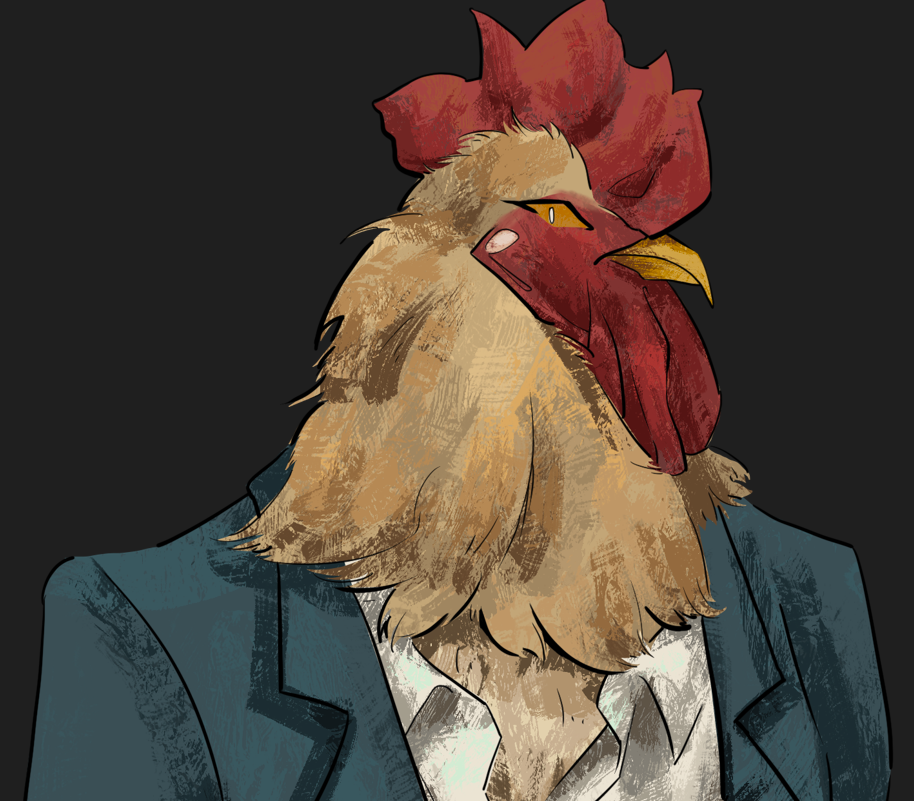
\includegraphics[width=0.3\textwidth]{Images/信存者/siyu.png}}
\subfigure[活泼的对比色]{
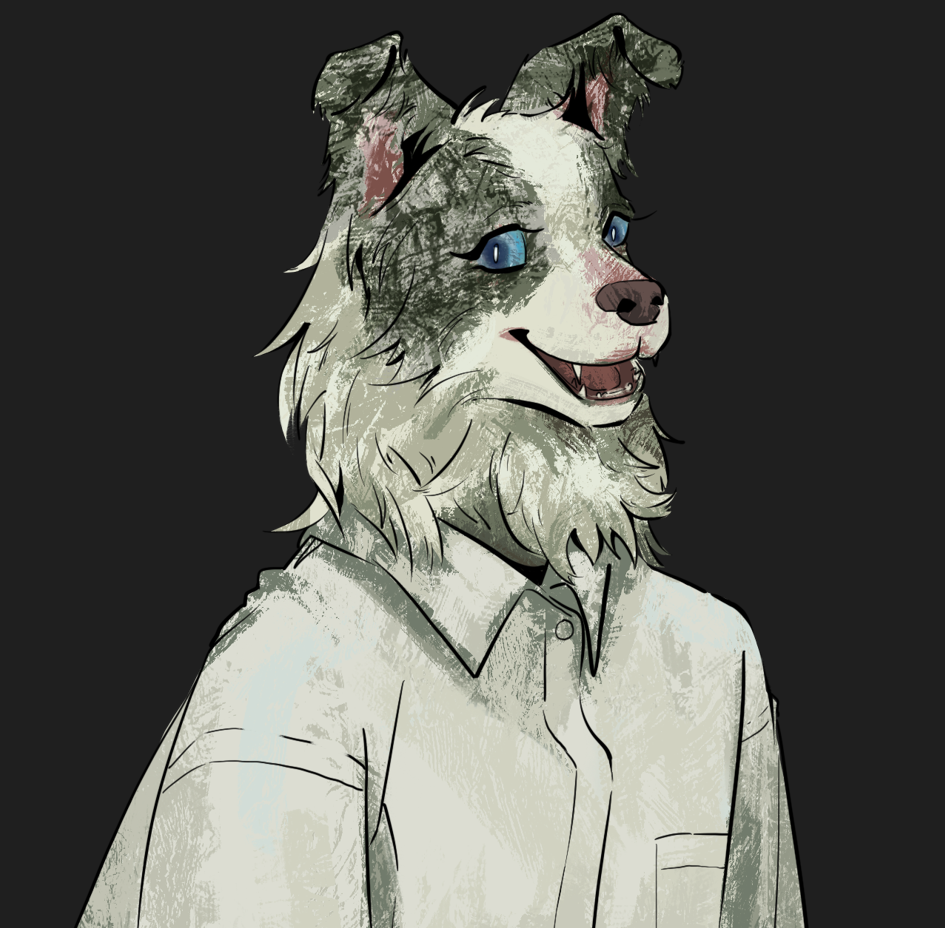
\includegraphics[width=0.3\textwidth]{Images/信存者/bei.png}}
\caption{性格迥异的动物角色设计}
\end{figure}

为了快速完成迭代,我们学习了《人生重开模拟器》的源代码,进行了配表,大大优化游戏迭代流程。

\begin{figure}[H]
    \centering  %图片全局居中
    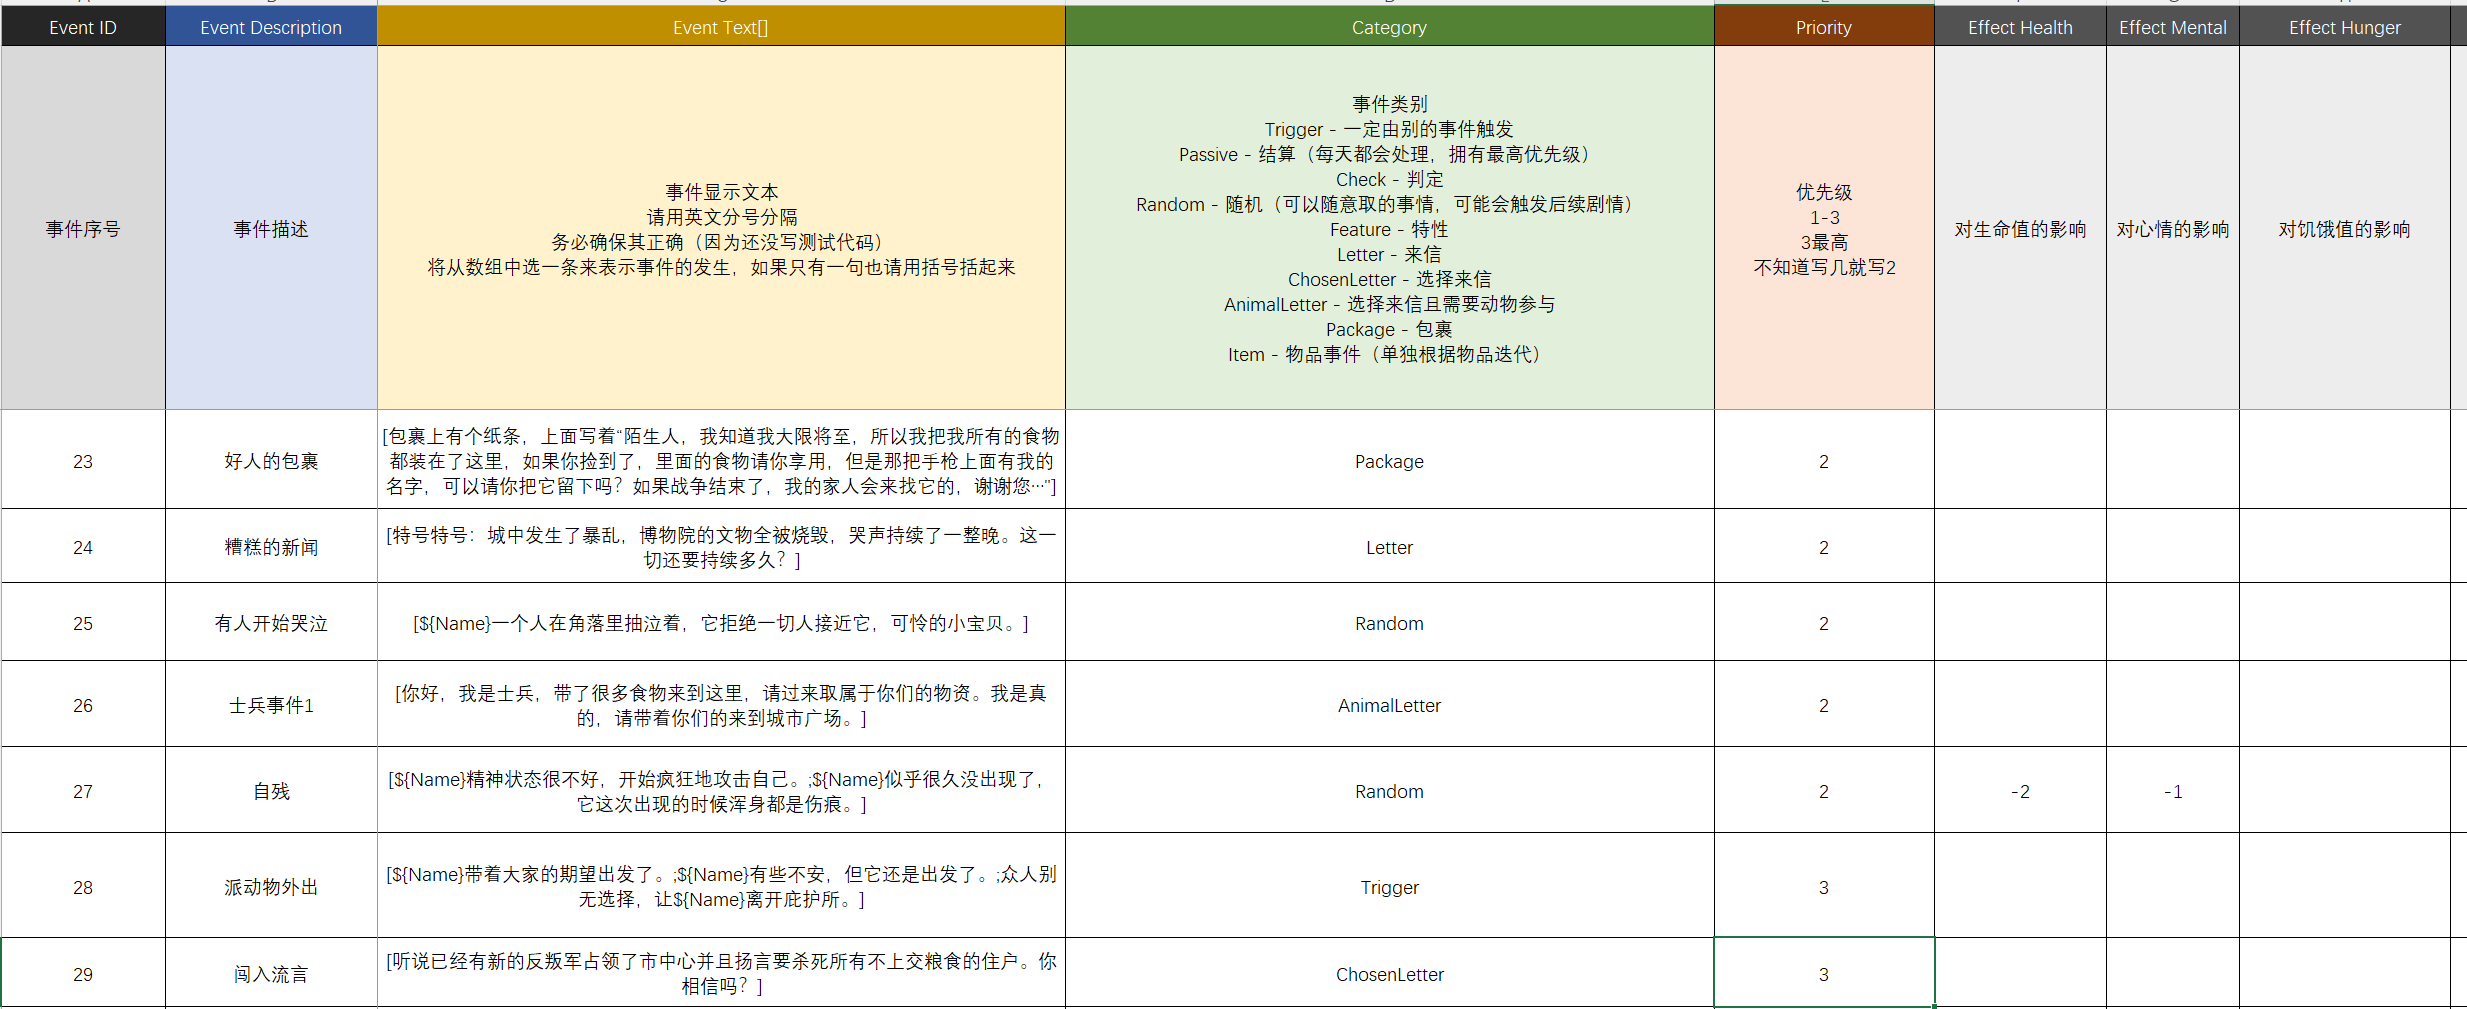
\includegraphics[width=0.9\textwidth]{Images/信存者/table_event.png}
    \caption{事件配表}
\end{figure}




\section{演示链接}
\begin{itemize}
    \item \textbf{试玩视频:}  \href{https://www.bilibili.com/video/BV1iY411q7mY/?vd_source=ead0ac501dfae814e19fd7d9f376d92d}{Bilibili视频}
    \item \textbf{Demo下载:}  \href{https://scyq.itch.io/creditors}{itch.io界面} 
    \item \textbf{网易Mini-Game参赛页面:} \href{https://game.academy.163.com/event/mg-2022?page=works&id=2838}{作品链接}
\end{itemize}
